\graphicspath{{content/1_literatureReview/figures/}}
\section{Current sensing}\label{sec:cursens}

\subsubsection{Sensing Techniques}\label{sec:cur_sum}
Measurement techniques are usually either "invasive" or "non-invasive". Invasive techniques tap into the circuit directly and often have a significant affect
on its operation, whereas non-invasive techniques might use e.g. the circuit's magnetic flux to determine the strength of the current.
A list of a few of these techniques \cite{currentSenseMethods} include:
\begin{itemize}
    \item A current-sensing resistor in series, which uses Ohm's law with a voltage measurement to calculate current.
    \item Hall element sensors, which determine the strength of current based on how much its magnetic field "bends" another current left and right (which creates a potential difference).
    \item Coil techniques, which make using of Faraday's law.
\end{itemize}

\begin{figure}[h!]
    \centering
    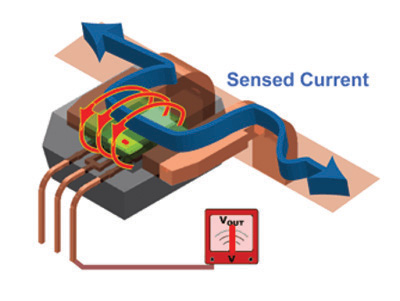
\includegraphics[width=.3\linewidth]{currentSensing_hall_effect}
    \captionof{figure}{Illustration of Hall Effect Sensors}
    \label{fig:hall-effect}
  \end{figure}

\subsubsection{High-side vs low-side sensing}\label{sec:cur_highlow}
These names of these two techniques refer to the placement of a current-sense resistor relative to the load. For circuits which draw higher currents, high-side sensing can be used
(placing the resistor closer to the positive of the voltage source) and is often more convenient. Low-side sensing, on the other hand, can potentially cause ground loop
issues \cite{currentSenseLowHighSide}, but has the ability to detect faults earlier.

\subsubsection{AC, DC, and Power Requirements}\label{sec:cur_acdc}
As mentioned, there are various non-invasive and even wireless techniques used to measure current. Faraday's law is used to make measurements using induction, which requires AC.
The Hall effect and sense resistors, on the other hand, are often used in the DC case. Wireless techniques have benefits over resistors in that they can be configured to draw much less power,
whereas sense resistors usually need high power handling capabilities as they pass through all current drawn by the actual load.
